\documentclass[]{beamer}
%\documentclass[notes]{beamer}
\usepackage{pgfpages}
%\setbeameroption{show notes on second screen}
%\setbeamertemplate{note page}[plain]
\usepackage{minted}
\usepackage{mathtools}
\usepackage{cancel}

\usetheme{UiB}
\setbeamertemplate{navigation symbols}{}
\usepackage{quantikz}
\usepackage{booktabs}
\usepackage{inconsolata}
\usepackage{physics}
\usetikzlibrary{shapes}

\newcommand{\code}[1]{\texttt{#1}}

\newcommand{\source}[1]{%
    \setbeamertemplate{footnote}[unnumbered]%
    \footnotetext{#1}%
}

\title{Quantum Computing (Lab)}
\author{Tutor: Massimiliano Incudini}
\institute{Università degli Studi di Verona}
\date{\today}

\begin{document}

%\section{Lecture 1}
\SectionPage{}

\begin{frame}{The scenario}
    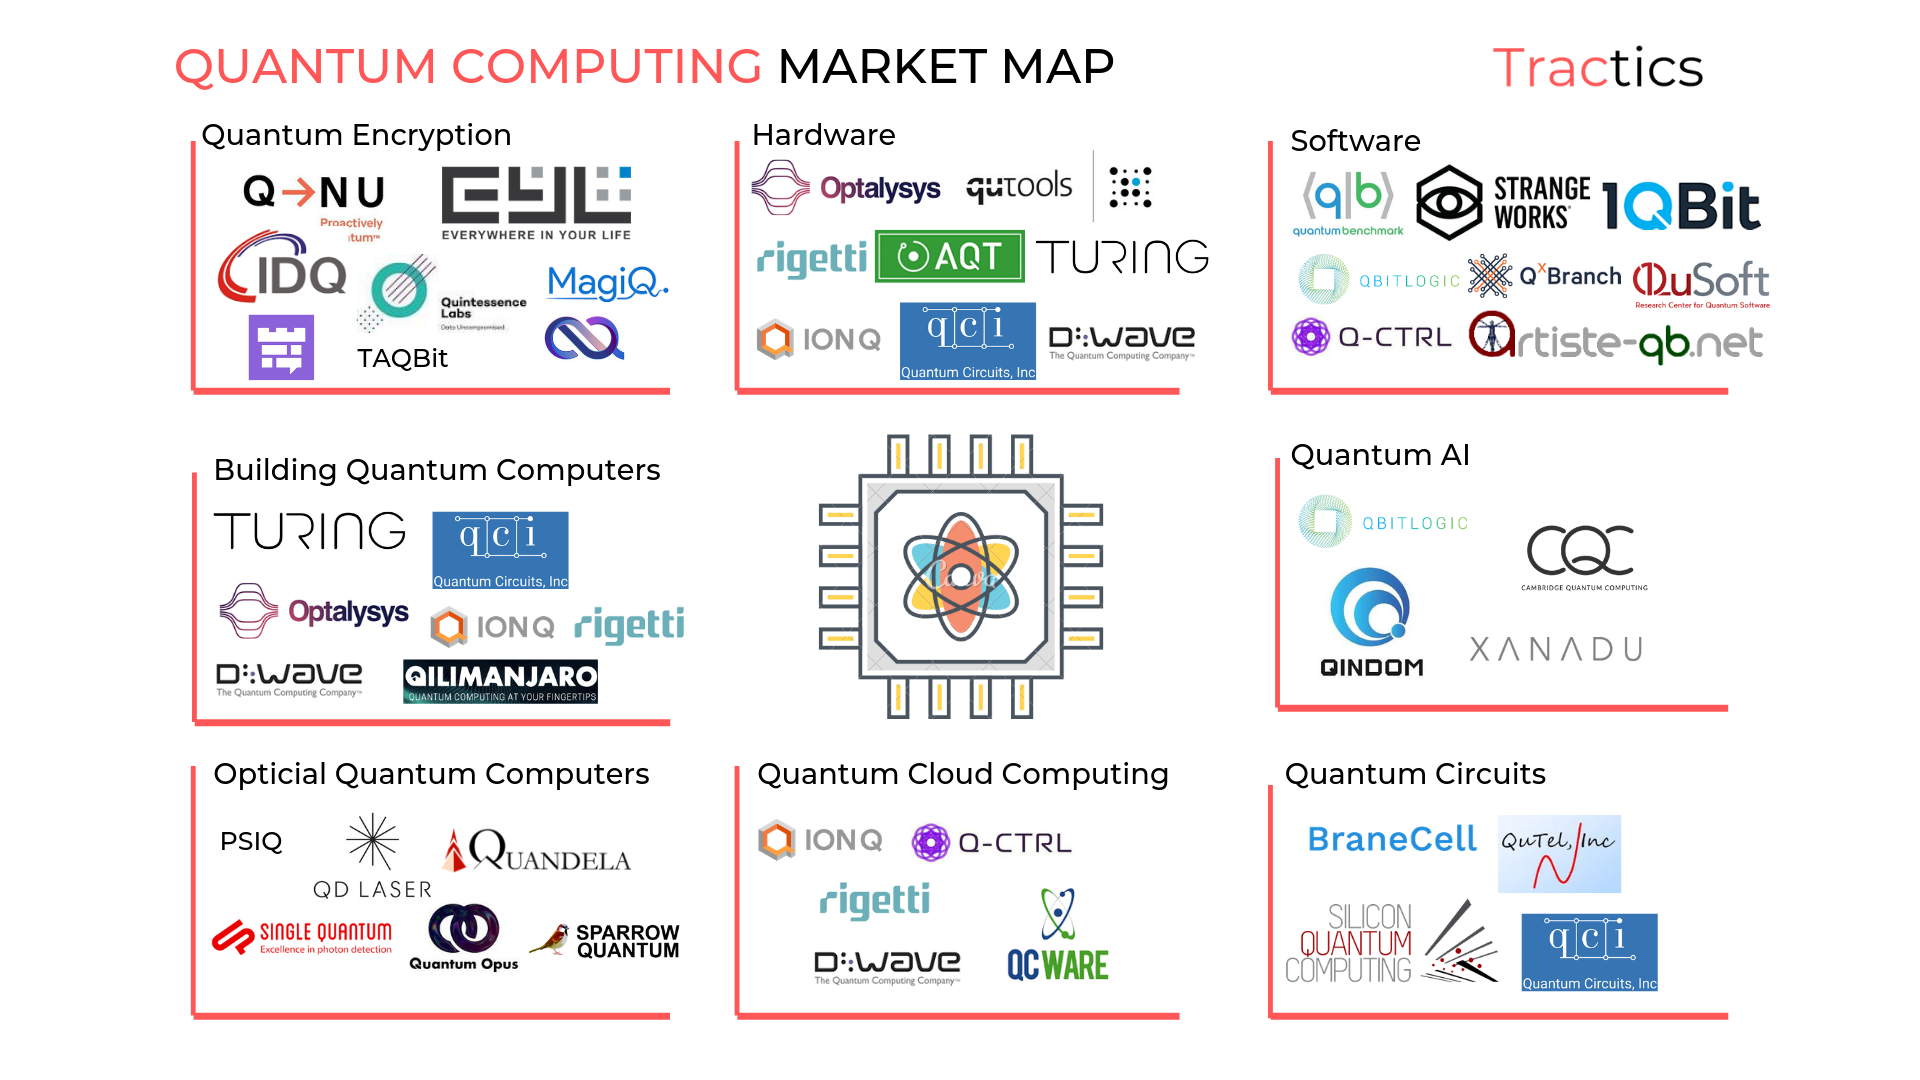
\includegraphics[width=\textwidth]{img/lec1/qc_landscape.png}
\end{frame}


\begin{frame}{The scenario}
    
\includegraphics[width=\textwidth]{img/lec1/qc_landscape_zoom.png}
\end{frame}

\begin{frame}{How to install}
\begin{itemize}
    \item<1-> \url{https://youtu.be/aYCjWymN_Hk}
    \item<2-> Windows, Mac, Linux
    \item<3-> Python 3 + Anaconda + pip + Qiskit
\end{itemize}
\end{frame}


\begin{frame}[fragile]{Check your installation}
\begin{minted}{Python}
import qiskit
qiskit.__qiskit_version__
# {'qiskit-terra': '0.16.1',
#  'qiskit-aer': '0.7.2',
#  'qiskit-ignis': '0.5.1',
#  'qiskit-ibmq-provider': '0.11.1',
#  'qiskit-aqua': '0.8.1',
#  'qiskit': '0.23.2'}
\end{minted}
\end{frame}


\begin{frame}{Qiskit platform}
\begin{itemize}
    \item<1-> \emph{Terra}: circuit definition
    \item<2-> \emph{Aer}: simulation and execution
    \item<3-> \emph{Ignis}: error mitigation and correction
    \item<4-> \emph{Aqua}: algorithms for machine learning, optimization, finance, chemistry
\end{itemize}
\end{frame}



\begin{frame}{The Quantum Circuit}
\begin{itemize}
    \item<1-> define the circuit (\code{QuantumCircuit})
    \begin{itemize}
        \item<2-> 1+ \code{QuantumRegister} (w/ optional name)
        \item<3-> 0+ \code{ClassicalRegister} (w/ optional name)
    \end{itemize}
    \item<4-> draw the circuit (method \code{draw} of \code{QuantumCircuit})
    \item<5-> add the gates (methods of \code{QuantumCircuit})
    \begin{itemize}
        \item<6-> \code{.x(qubit)}
        \item<8-> \code{.h(qubit)}
        \item<9-> \code{.cx(control qubit, target qubit)}
        \item<10-> \code{.rx(theta, qubit)}
        \item<11-> \code{.crx(theta, control qubit, target qubit)}
        \item<12-> optionally use indexes instead of qubit
        \begin{itemize}
            \item<13-> depends on the order you insert the registers
            \item<14-> be consistent w/ the notation
        \end{itemize}
    \end{itemize}
    \item<15-> add the measurements (method of \code{QuantumCircuit})
    \begin{itemize}
        \item<15-> \code{.measure(qubit, cbit)}
    \end{itemize}
\end{itemize}
\end{frame}


\begin{frame}[fragile]{The code (1)}
\begin{minted}{python}
from qiskit import *

# first circuit
qr = QuantumRegister(2, 'qreg')
qc = QuantumCircuit(qr)
qc.draw()

qc.h(qr[0])
qc.cx(qr[0], qr[1])
qc.rx(0.1, qr[1])
qc.draw()
\end{minted}
\end{frame}


\begin{frame}[fragile]{The code (2)}
\begin{minted}{python}
# second circuit
qra = QuantumRegister(2, 'qa')
qrb = QuantumRegister(2, 'qb')
cr = ClassicalRegister(2, 'creg')
qc = QuantumCircuit(qra, qrb, cr)
qc.cx(qra[0], qra[1])
qc.cy(qrb[0], qrb[1])
qc.cx(0, 1)
qc.cy(2, 3)
qc.measure(0, 0)
qc.draw()
\end{minted}
\end{frame}

\begin{frame}{Simulators}
\begin{itemize}
    \item<1-> \emph{Statevector simulator}: output the complex vector of amplitudes
    \item<2-> \emph{Unitary simulator}: output the complex matrix representing the transformation performed by your circuit
    \item<3-> \emph{``QASM" simulator}: mime the behaviour of the real hardware, output the distribution of the possible outcomes
    \begin{itemize}
        \item<4-> error due to probabilistic nature of the processing
        \item<5-> \(\neq\) noise (which can be simulated too)
    \end{itemize}
\end{itemize}
\end{frame}

\begin{frame}[fragile]{The code (3)}
\begin{minted}{python}
from qiskit import Aer
Aer.backends()

statevector_sim = Aer.get_backend('statevector_simulator')
unitary_sim = Aer.get_backend('unitary_simulator')
qasm_sim = Aer.get_backend('qasm_simulator')

qc = QuantumCircuit(2, 2)
qc.h(0)
qc.cx(0, 1)

result = execute(qc, backend=statevector_sim, shots=1).result()
    .get_statevector()
# array([0.70710678+0.j, 0.        +0.j, 
#        0.        +0.j, 0.70710678+0.j])

result = execute(qc, backend=unitary_sim, shots=1).result().get_unitary()
# array([[ 0.70710678+0.00000000e+00j,  0.70710678-8.65956056e-17j,
#          0.        +0.00000000e+00j,  0.        +0.00000000e+00j],
#        [ 0.        +0.00000000e+00j,  0.        +0.00000000e+00j,
#          0.70710678+0.00000000e+00j, -0.70710678+8.65956056e-17j],
#        [ 0.        +0.00000000e+00j,  0.        +0.00000000e+00j,
#          0.70710678+0.00000000e+00j,  0.70710678-8.65956056e-17j],
#        [ 0.70710678+0.00000000e+00j, -0.70710678+8.65956056e-17j,
#          0.        +0.00000000e+00j,  0.        +0.00000000e+00j]])

result = execute(qc, backend=qasm_sim, shots=1000).result().get_counts()
# {'00': 1000}

qc.measure(0, 0)
qc.measure(1, 1)
result = execute(qc, backend=qasm_sim, shots=1000).result().get_counts()
# {'00 00': 506, '11 00': 494}
\end{minted}
\end{frame}


\begin{frame}[fragile]{The code (4)}
\begin{minted}{python}
result = execute(qc, backend=unitary_sim, shots=1).result()
    .get_unitary()
# array([
#  [ 0.70710678+0.00000000e+00j,  0.70710678-8.65956056e-17j,
#    0.        +0.00000000e+00j,  0.        +0.00000000e+00j],
#  [ 0.        +0.00000000e+00j,  0.        +0.00000000e+00j,
#    0.70710678+0.00000000e+00j, -0.70710678+8.65956056e-17j],
#  [ 0.        +0.00000000e+00j,  0.        +0.00000000e+00j,
#    0.70710678+0.00000000e+00j,  0.70710678-8.65956056e-17j],
#  [ 0.70710678+0.00000000e+00j, -0.70710678+8.65956056e-17j,
#    0.        +0.00000000e+00j,  0.        +0.00000000e+00j]
# ])
\end{minted}
\end{frame}


\begin{frame}[fragile]{The code (5)}
\begin{minted}{python}
result = execute(qc, backend=qasm_sim, shots=1000).result()
    .get_counts()
# {'00': 1000}

qc.measure(0, 0)
qc.measure(1, 1)
result = execute(qc, backend=qasm_sim, shots=1000).result()
    .get_counts()
# {'00': 503, '11': 497}
\end{minted}
\end{frame}

\begin{frame}{Bloch sphere}
\begin{itemize}
    \item<1-> Visualize single qubit transformations
    \item<2-> \code{kaleidoscope} library
    \item<3-> input \(=\) vector representing the quantum state
    \item<4-> interactive!
\end{itemize}

\begin{center}
    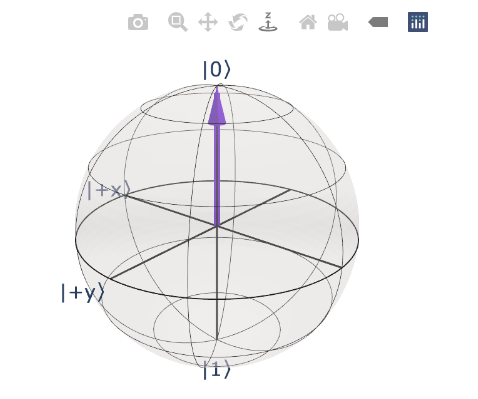
\includegraphics[width=0.5\textwidth]{img/lec1/bloch_sphere.png}
\end{center}
\end{frame}

\begin{frame}[fragile]{The code (6)}
\begin{minted}{python}
!pip install kaleidoscope
from kaleidoscope import bloch_sphere
from qiskit.quantum_info import Statevector
qc = QuantumCircuit(1)
figure = bloch_sphere(Statevector.from_instruction(qc))
figure.show()
\end{minted}
\end{frame}

% https://github.com/Qiskit/qiskit-tutorials/blob/master/tutorials/circuits_advanced/01_advanced_circuits.ipynb

\begin{frame}{Arbitrary initialization}
Encode a complex vector of \(2^n\) in a \(n\)-qubit register.
\end{frame}

\begin{frame}[fragile]{The code (7)}
\begin{minted}{python}
import numpy as np
amplitudes = np.array([1+0j, 2+2j, 3+4j, 6+0.55j])
amplitudes = amplitudes / np.linalg.norm(amplitudes)
# np.linalg.norm(amplitudes) = 0.9999999999999999
amplitudes = amplitudes / np.linalg.norm(amplitudes)
# np.linalg.norm(amplitudes) = 1.0

qc = QuantumCircuit(2)
qc.initialize(amplitudes)
\end{minted}
\end{frame}

\begin{frame}{Transpiling}
Given 
\begin{itemize}
    \item a circuit
    \item an universal set on ``known" gates
    \item a topology (pairs of adjacent qubits)
\end{itemize}
construct a circuit equivalent which can be run on the given configuration.

\only<2->{\bigskip Different (real) machines have different configurations, and the transpiling operation will lead to different circuits. }
\end{frame}

\begin{frame}[fragile]{The code (8)}
\begin{minted}{python}
qc = QuantumCircuit(2)

amp = array([0.11926544+0.j, 0.23853088+0.23853088j, 
             0.35779632+0.47706176j, 0.71559264+0.06559599j])
qc.initialize(amp)
qc.size() # 1

qc2 = transpile(qc, basis_gates=['u3', 'cx'])
qc2.size() # 6
\end{minted}
\end{frame}

\begin{frame}[fragile]{Execution on IBM machines}

Register on IBMQ, then visit \url{https://quantum-computing.ibm.com/account} and copy your token. Then execute (once): \medskip

\begin{minted}{python}
from qiskit import IBMQ
IBMQ.save_account('insert_token_here')
\end{minted}

\medskip Finally access your real backends through:\medskip

\begin{minted}{python}
IBMQ.load_account()
provider = IBMQ.get_provider()
# provider.backends() lists the available machines
backend = provider.get_backend('ibmq_santiago')
counts = execute(qc, backend, shots=1000).result().get_counts()
\end{minted}

\medskip Additional information on \url{github.com/Qiskit/qiskit-ibmq-provider}. 
\end{frame}

\begin{frame}{OpenQASM format}
Intermediate representation for quantum instructions. 

\only<2->{\bigskip Most circuit-based quantum computing framework can import and export from/to OpenQASM.}

\only<3->{\bigskip Try method \code{.qasm} of \code{QuantumCircuit}}
\end{frame}

\begin{frame}{Your turn!}
\begin{itemize}
    \item<1-> Check your Qiskit installation!
    \item<2-> Define the circuits implementing the Bell states, simulate and execute them with any backend seen so far (including real machines)
    \item<3-> Tell me: how much the circuit size for arbitrary initialization grows when the number of qubit grows?
    \item<4-> Try Deutsch-Jozsa (\url{qiskit.org/textbook/ch-algorithms/deutsch-jozsa.html})
    \item<5-> Open \url{qiskit.org/documentation/tutorials.html}
\end{itemize}
\end{frame}


%\section{Lecture 2: \\ Quantum Protocols}
\SectionPage{}

\begin{frame}{Quantum Teleportation}

\bigskip

The IBM quantum computers currently do not support instructions after measurements, meaning we cannot run the quantum teleportation in its current form on real hardware. 

\bigskip

\begin{definition}[Principle of deferred measurement]
Measurements can always be moved from an intermediate stage of a quantum circuit to the end of the circuit.

If the measurement results are used at any stage of the circuit then the \alert{classically controlled operations} can be replaced by \alert{conditional quantum operations}.
\end{definition}

\end{frame}

\begin{frame}{Deferred Measurement}
 
 A consequence of the principle of deferred measurement is that \alert{measurement commutes with control}.
 
 \bigskip
 
\begin{center}
    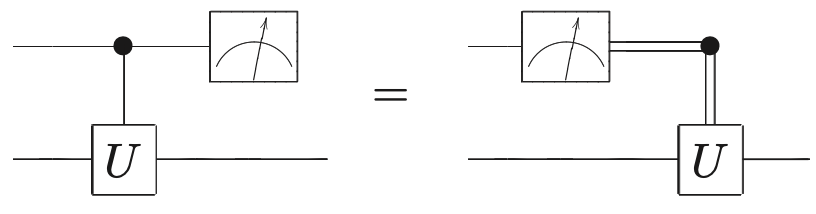
\includegraphics[width=0.85\textwidth]{img/DeferredMeasure.png}
\end{center}

\bigskip

\textbf{Exercise}

Prove the equality of the two circuits depicted above.


\end{frame}

\begin{frame}{Equivalent Teleportation Circuits}
 
\begin{center}
    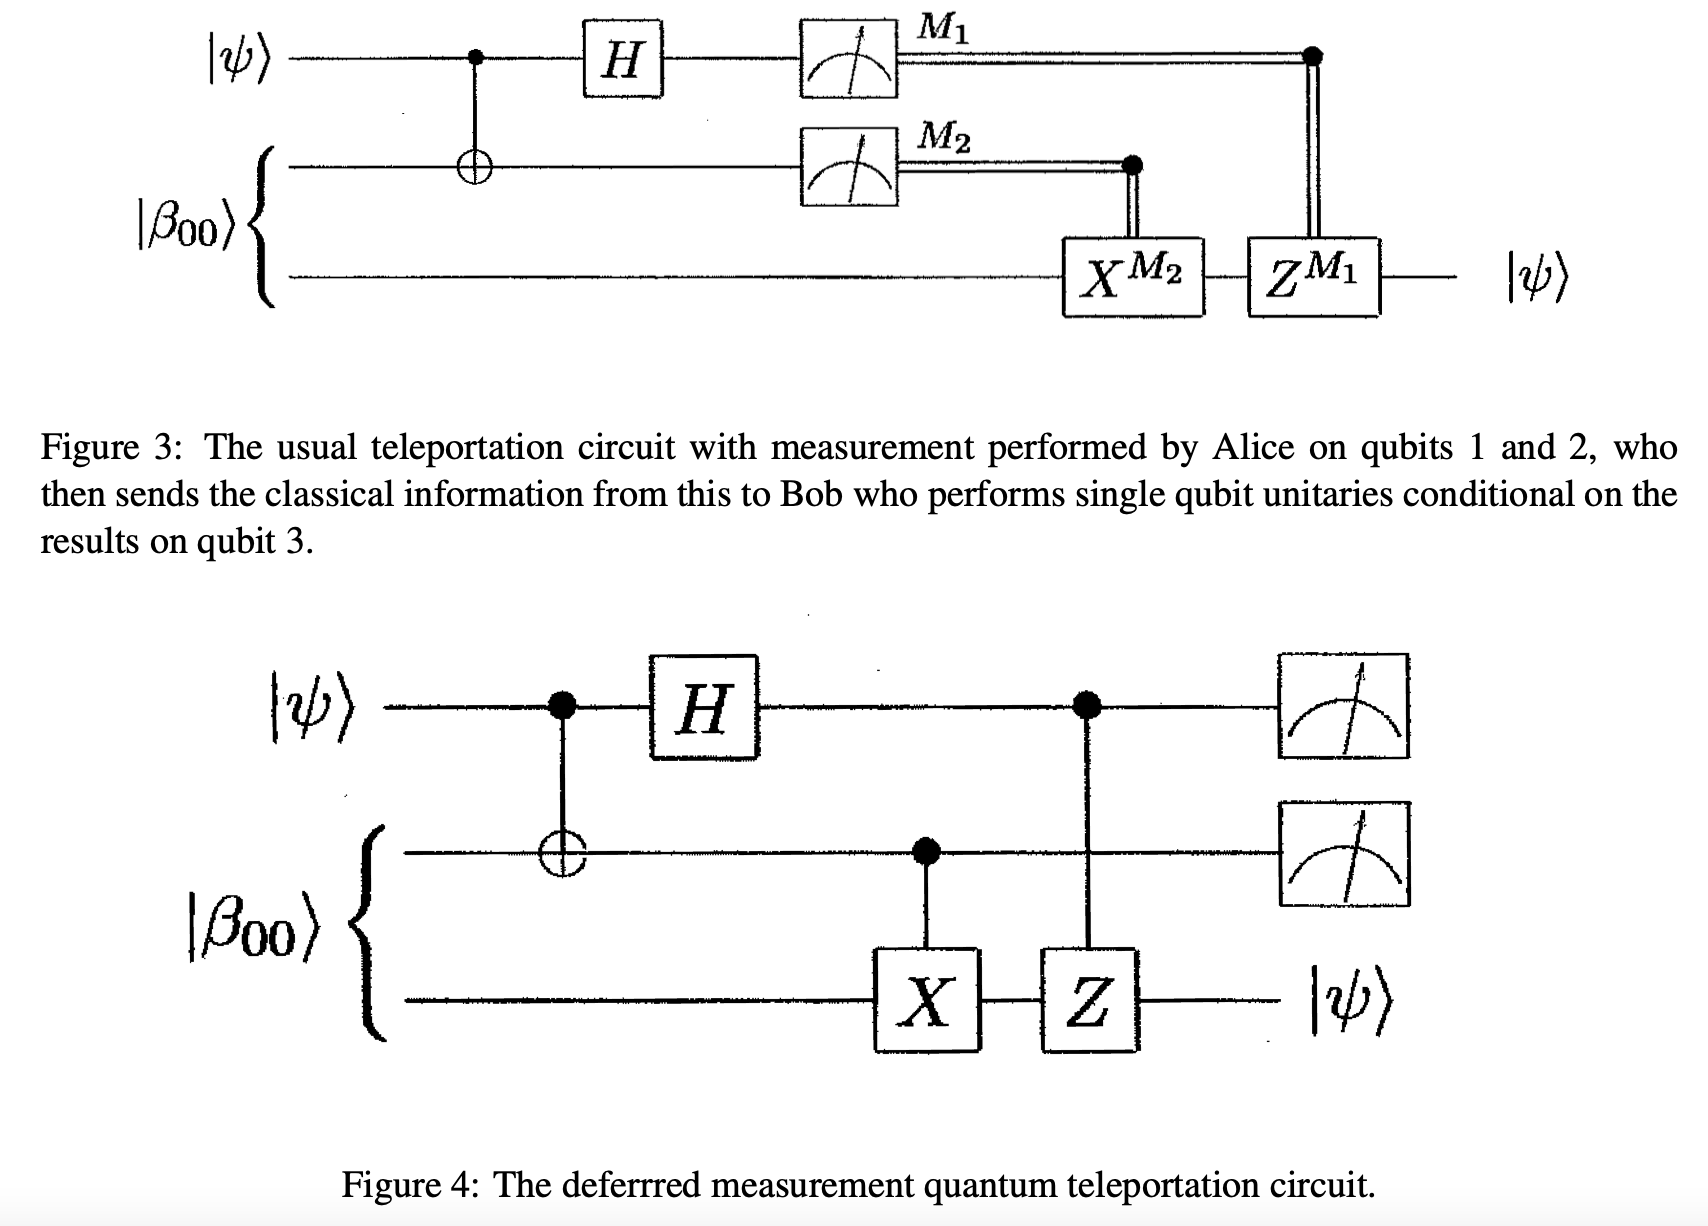
\includegraphics[width=0.80\textwidth]{img/EqivTelCircuits.png}
\end{center}
\end{frame}

\begin{frame}{Teleportation as State Transfer}
We are only interested in taking the input qubit $\psi$ to another location. We do not care what state we get in place of the original qubit at the sender. 

\begin{center}
    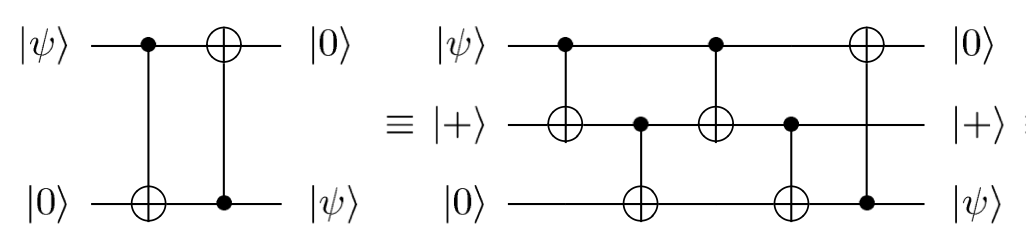
\includegraphics[width=0.80\textwidth]{img/state-transfer.png}
\end{center}

Other equivalent circuits:
\begin{center}
    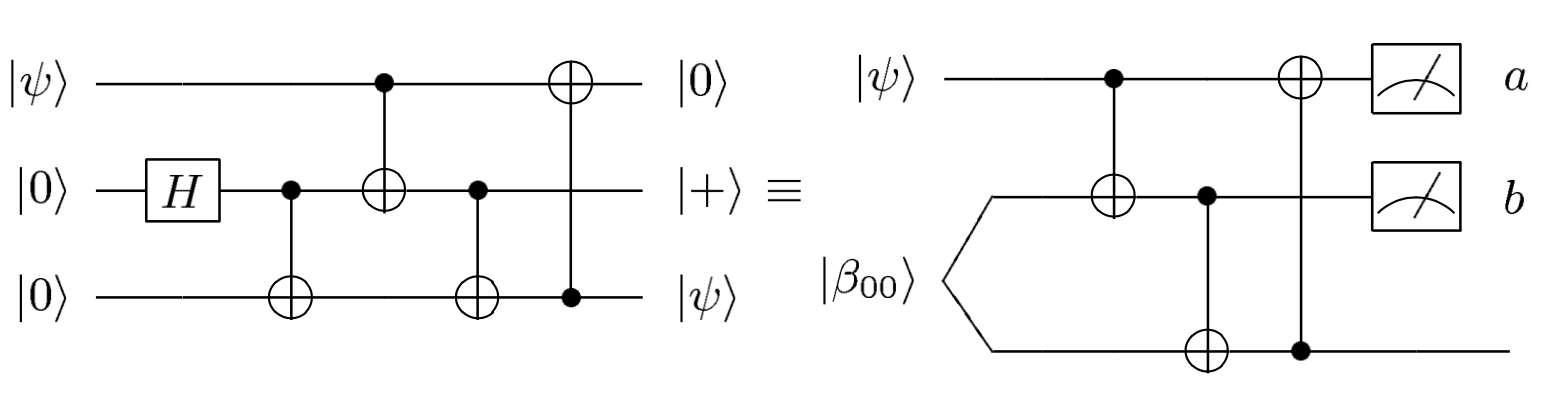
\includegraphics[width=0.80\textwidth]{img/Other-teleportation.png}
\end{center}
\end{frame}

\section{Exercise checking}
\SectionPage{}

% ============================================

\begin{frame}[fragile]{Exercise checking (1)}

\begin{itemize} 
\item Check your Qiskit installation
\end{itemize}

\begin{minted}{python}
import qiskit
qiskit.__qiskit_version__
\end{minted}

\bigskip No errors must appear (except the one regarding \code{matplotlib}, depending on the console you're using). 

\end{frame}

% ============================================

\begin{frame}[fragile]{Exercise checking (2)}

\begin{itemize} 
\item Define the circuits implementing the Bell states, simulate and execute them with any backend seen so far (including real machines)
\end{itemize}

\begin{minted}{python}
qc = QuantumCircuit(2, 2)
qc.h(0)
qc.cx(0, 1)

statevector_sim = Aer.get_backend('statevector_simulator')
statevector_result = execute(qc, backend=statevector_sim, shots=1)
    .result().get_statevector()

unitary_sim = Aer.get_backend('unitary_simulator')
unitary_result = execute(qc, backend=unitary_sim, shots=1)
    .result().get_unitary()
\end{minted}

\end{frame}


\begin{frame}[fragile]{Exercise checking (2)}

\begin{itemize} 
\item Define the circuits implementing the Bell states, simulate and execute them with any backend seen so far (including real machines)
\end{itemize}

\begin{minted}{python}
qc.measure([0, 1], [0, 1])
qasm_sim = Aer.get_backend('qasm_simulator')
qasm_result = execute(qc, backend=qasm_simulator, shots=1000)
    .result().get_statevector()

IBMQ.load_account()
santiago = IBMQ.get_provider().get_backend('ibmq_santiago')
counts = execute(qc, backend=santiago, shots=1000).result().get_counts()
\end{minted}

\end{frame}

% ============================================

\begin{frame}[fragile]{Exercise checking (3)}

\begin{itemize} 
\item How does the circuit size for arbitrary initialization grow when the number of qubit increases?
\end{itemize}

\begin{minted}{python}
from qiskit import * 
from qiskit.quantum_info.states.random import random_statevector

qubits = [1, 2, 3, 4, 5, 6, 7, 8]
sizes = []

for qubit in qubits:
	qc = QuantumCircuit(qubit)
	statevector = random_statevector(2**qubit)
	qc.initialize(statevector.data)
	qc2 = transpile(qc, basis_gates=['u3','cx'])
	sizes.append(qc2.size())
	
# sizes = [1, 6, 19, 48, 109, 234, 487, 996]
\end{minted}

\end{frame}


% ============================================

\begin{frame}[fragile]{Exercise checking (4)}

\begin{itemize} 
\item Try Deutsch-Jozsa
\end{itemize}

\bigskip See \url{qiskit.org/textbook/ch-algorithms/deutsch-jozsa.html}.

\end{frame}


\section{Quantum Teleportation}
\SectionPage{}

\begin{frame}{A note on Qiskit: which qubit is leftmost?}

\begin{center}
\begin{quantikz}[]
\lstick{\(\ket{\psi}\)}\qw
    & \gate[wires=3]{teleport}
    & \qw\rstick{\(\ket{b_1}\)} \\
\lstick{\(\ket{0}\)}\qw
    & \qw
    & \qw\rstick{\(\ket{b_2}\)} \\
\lstick{\(\ket{0}\)}\qw
    & \qw
    & \qw\rstick{\(\ket{\psi}\)}
\end{quantikz}
\end{center}

\bigskip At the beginning of the circuit the state is \( \ket{0} \otimes \ket{0} \otimes \ket{\psi} \)

\bigskip At the end of the circuit the state is \( \ket{\psi} \otimes \ket{b_2} \otimes \ket{b_1} \)

\end{frame}

% =====================================================

\begin{frame}[fragile]{The code (1)}

\begin{minted}[fontsize=\footnotesize]{python}
from qiskit.quantum_info.states.random import random_statevector
from qiskit import * \ import numpy as np

psi = random_statevector(2).data  
# array([0.75160912+0.04778984j, 0.49917654-0.42851213j])
qc = QuantumCircuit(3, 3)
qc.initialize(psi, 0)
sv_sim = Aer.get_backend('statevector_simulator')
statevector = execute(qc, sv_sim).result().get_statevector()
# array([0.75160912+0.04778984j, 0.49917654-0.42851213j,
#        0.        +0.j        , 0.        +0.j        ,
#        0.        +0.j        , 0.        +0.j        ,
#        0.        +0.j        , 0.        +0.j        ])
ket_zero = np.array([1, 0])
np.kron(np.kron(ket_zero, ket_zero), psi)
# array([0.75160912+0.04778984j, 0.49917654-0.42851213j,
#        0.        +0.j        , 0.        +0.j        ,
#        0.        +0.j        , 0.        +0.j        ,
#        0.        +0.j        , 0.        +0.j        ])
\end{minted}

\end{frame}


\begin{frame}{The protocol (1)}
\begin{quantikz}[]
\lstick[wires=2]{Alice}\qw
    & \gate{init(\ket{\psi})}
    & \qw \\
    \qw
    & \qw
    & \qw \\
\lstick{Bob}\qw
    & \qw
    & \qw
\end{quantikz}

\bigskip Alice own the qubit in state \(\ket{\psi} = \alpha \ket{0} + \beta \ket{1}\)
\end{frame}

% =========================================

\begin{frame}{The protocol (2)}
    
\begin{quantikz}[]
\lstick[wires=2]{Alice}\qw
    & \gate{init(\ket{\psi})}
    & \qw \\
    \qw
    & \gate[wires=2]{bell}
    & \qw\\
\lstick{\(\ket{0}\)}\qw
    & \qw
    & \qw
\end{quantikz}

\bigskip Alice and Bob shares a Bell state \(\frac{1}{\sqrt{2}} (\ket{00} + \ket{11})\)
\end{frame}

% =========================================

\begin{frame}[fragile]{Composed gates}

Hierarchical organization of the circuit

\begin{minted}{python}
def create_bell_circuit():
	bell_circuit = QuantumCircuit(2, name='bell')
	bell_circuit.h(0)
	bell_circuit.cx(0, 1)
	return bell_circuit

psi = random_statevector(2).data
qr = QuantumRegister(3, 'q')
crx = ClassicalRegister(1, 'crx')
crz = ClassicalRegister(1, 'crz')
qc = QuantumCircuit(qr, crx, crz)
qc.initialize(psi, qr[0])
qc.append(create_bell_circuit(), [qr[0], qr[1]])
\end{minted}
\end{frame}

% =========================================

\begin{frame}{The protocol (3)}
    
\begin{quantikz}[]
\lstick[wires=2]{Alice}\qw
    & \gate{init(\ket{\psi})}
    & \ctrl{1} 
    & \gate{H} 
    & \qw \\
    \qw
    & \gate[wires=2]{bell}
    & \targ{}
    & \qw
    & \qw\\
\lstick{\(\ket{0}\)}\qw
    & \qw
    & \qw
    & \qw
    & \qw
\end{quantikz}

\bigskip Alice applies CNOT and H, the state becomes
\begin{align*}
    \frac{1}{2} \Big( & \ket{00}(\alpha \ket{0} + \beta \ket{1}) \\
                    + & \ket{01}(\alpha \ket{1} + \beta \ket{0}) \\
                    + & \ket{10}(\alpha \ket{0} - \beta \ket{1}) \\
                    + & \ket{10}(\alpha \ket{1} - \beta \ket{0})\Big) 
\end{align*}
\end{frame}

% =========================================

\begin{frame}{The protocol (4)}
    
\begin{quantikz}[]
\lstick[wires=2]{Alice}\qw
    & \gate{init(\ket{\psi})}
    & \ctrl{1} 
    & \gate{H} 
    & \meter{}
    & \cw
    & \cwbend{2}\\
    \qw
    & \gate[wires=2]{bell}
    & \targ{}
    & \qw
    & \meter{}
    & \cwbend{1} \\
\lstick{\(\ket{0}\)}\qw
    & \qw
    & \qw
    & \qw
    & \qw
    & \gate{X}
    & \gate{Z}
    & \qw
\end{quantikz}

\bigskip Alice measures and send the two classical bits, Bob adjusts its qubit according to the received bits:
\begin{align*}
    00 & \to I \\
    01 & \to X \\
    10 & \to Z \\
    11 & \to ZX
\end{align*}
\end{frame}

% =========================================

\begin{frame}[fragile]{The code (2)}
\begin{minted}{python}
psi = random_statevector(2).data

qr = QuantumRegister(3, 'q')
crx = ClassicalRegister(1, 'crx')
crz = ClassicalRegister(1, 'crz')
qc = QuantumCircuit(qr, crx, crz)
qc.initialize(psi, qr[0])
qc.append(create_bell_circuit(), [qr[1], qr[2]])

qc.cx(qr[0], qr[1])
qc.h(qr[0])
qc.measure(qr[0], crz)
qc.measure(qr[1], crx)
qc.x(qr[2]).c_if(crx, 1)
qc.z(qr[2]).c_if(crz, 1)
\end{minted}
\end{frame}

\begin{frame}[fragile]{The code (3)}
\begin{minted}{python}
sv_sim = Aer.get_backend('statevector_simulator')
sv = execute(qc, sv_sim).result().get_statevector()
\end{minted}

\bigskip Is \code{sv} the state \( \ket{\psi} \otimes \ket{b_2} \otimes \ket{b_1} \)?
\end{frame}

% =========================================

\begin{frame}[fragile]{The code (4)}

What is we use deferred measurements? \bigskip

\begin{minted}{python}
qr = QuantumRegister(3, 'q')
crx = ClassicalRegister(1, 'crx')
crz = ClassicalRegister(1, 'crz')
qc = QuantumCircuit(qr, crx, crz)
qc.initialize(psi, qr[0])
qc.append(create_bell_circuit(), [qr[1], qr[2]])

qc.cx(qr[0], qr[1])
qc.h(qr[0])
qc.cx(qr[0], qr[2])
qc.cz(qr[1], qr[2])
qc.measure(qr[0], crz)
qc.measure(qr[1], crx)
\end{minted}
\end{frame}

% =========================================

\begin{frame}{Running on real quantum computers}

\begin{itemize}
    \item Deferred measurement is mandatory;
    \item How can I check if the state is exactly the one Alice wanted to send?
\end{itemize}
\end{frame}

\begin{frame}{Running on real quantum computers}

\begin{itemize}
    \item Deferred measurement is mandatory;
    \item How can I check if the state is exactly the one Alice wanted to send?
\end{itemize}

\bigskip
\begin{center}
\begin{quantikz}[]
\lstick{\(\ket{0}\)}\qw
    & \gate{init}
    & \gate[wires=3]{teleport}
    & \qw \\
\lstick{\(\ket{0}\)}\qw
    & \qw
    & \qw
    & \qw \\
\lstick{\(\ket{0}\)}\qw
    & \qw
    & \qw
    & \gate{init^{-1}}
    & \qw\rstick{\(\ket{0}\)}
\end{quantikz}
\end{center}

\qquad Check if the last qubit is zero

\end{frame}

% =========================================

\begin{frame}[fragile]{Inverse of \code{initialize} gate}

\begin{minted}{python}
from qiskit.extensions import Initialize
psi = random_statevector(2).data

init_gate = Initialize(psi)
init_gate.label = 'init'

inverse_init_gate = init_gate.gates_to_uncompute()

qc = QuantumCircuit(1)
qc.append(init_gate, [0])
qc.append(inverse_init_gate, [0])
sv = execute(qc, sv_sim).result().get_statevector()
# sv is ALMOST ket zero
\end{minted}

\end{frame}

% =========================================

\begin{frame}[fragile]{Inverse of \code{initialize} gate}

Be careful: \code{initialize} contains a non-linear \code{Reset} gate \bigskip

\begin{minted}{python}
init_gate = Initialize(psi)
init_gate.inverse() # error

inverse_init_gate = init_gate.gates_to_uncompute() # no reset
init_wo_reset = inverse_init_gate.inverse()

init_wo_reset.inverse() # ok
\end{minted}

\end{frame}

\begin{frame}{More on Quantum Teleportation}
Check this video of \emph{minutephysics}: \url{youtube.com/watch?v=dAaHHGHuy1c}
\end{frame}

\begin{frame}{Your turn!}
\begin{itemize}
    \item Demonstrate the equivalence of these circuits:
    \begin{center}
        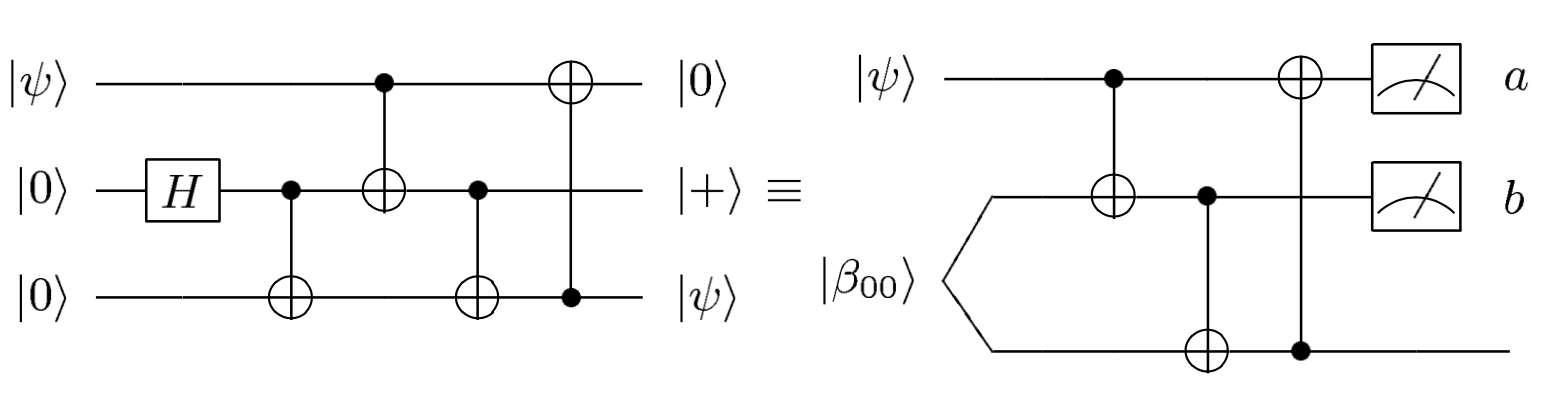
\includegraphics[width=0.80\textwidth]{img/Other-teleportation.png}
    \end{center}
    \item Run Quantum Teleportation
    \begin{itemize}
        \item \url{qiskit.org/textbook/ch-algorithms/teleportation.html}
        \item Explain how the network is used by Bob (Step 4) if the Bell state in input is $\frac{1}{\sqrt{2}}(\ket{01}+\ket{10})$.
    \end{itemize}
    \item Run Superdense Coding
    \begin{itemize}
        \item \url{qiskit.org/textbook/ch-algorithms/superdense-coding.html}
        \item Familiarize with the documentation!
    \end{itemize}
\end{itemize}

\end{frame}

% nota: eseguendo il circuito più volte il risultato dello statevector cambia, però facendo i conti sono i primi due qubit che cambiano e non il terzo
% controllare con metodo che fa 00psi, 01psi, 10psi, 11psi



%\section{Lecture 3: \\ Fourier Transform}
\SectionPage{}

\begin{frame}{Fourier Transform}
\begin{center}
    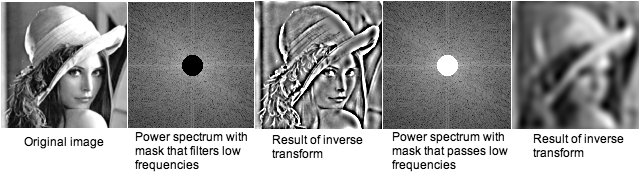
\includegraphics[width=\textwidth]{img/lec3/fft.jpg}
\end{center}
\end{frame}

\section{DFT}\SectionPage{}

\begin{frame}{DFT}
\onslide<1->{
\[
    \mqty[x_0 \\ x_1 \\ \vdots \\ x_{N-1}] 
    \xrightarrow{\text{DFT}}
    \mqty[y_0 \\ y_1 \\ \vdots \\ y_{N-1}] 
    \qquad 
    y_k = \frac{1}{\sqrt{N}} \sum_{j=0}^{N-1} x_j \; \exp(\frac{2\pi i}{N} \cdot j \cdot k)
\]}
\onslide<2->{
\[
    \mqty[y_0 \\ y_1 \\ \vdots \\ y_{N-1}] 
    \xrightarrow{\text{DFT}^{-1}}
    \mqty[x_0 \\ x_1 \\ \vdots \\ x_{N-1}] 
    \qquad 
    x_j = \frac{1}{\sqrt{N}} \sum_{k=0}^{N-1} y_k \; \exp(-\frac{2\pi i}{N} \cdot j \cdot k)
\]}
\end{frame}

% ===========================================

\begin{frame}{DFT}

\[
    \mqty[x_0 \\ x_1 \\ \vdots \\ x_{N-1}] 
    \xrightarrow{\text{DFT}}
    \mqty[y_0 \\ y_1 \\ \vdots \\ y_{N-1}] 
    \qquad 
    y_k = \frac{1}{\sqrt{N}} \sum_{j=0}^{N-1} x_j \; \alert{\omega}^{j \cdot k}
\]
\[
    \mqty[y_0 \\ y_1 \\ \vdots \\ y_{N-1}] 
    \xrightarrow{\text{DFT}^{-1}}
    \mqty[x_0 \\ x_1 \\ \vdots \\ x_{N-1}] 
    \qquad 
    x_j = \frac{1}{\sqrt{N}} \sum_{k=0}^{N-1} y_k \; \alert{\omega}^{-j \cdot k}
\]

\bigskip
\[ \alert{\omega} = \text{nth root of unity} \qquad \omega^{N+i}=\omega^i \]
\end{frame}

% ===========================================

\begin{frame}{DFT example}
Calculate \( \mqty[y_0 \\ y_1] = \mathrm{DFT}\left(\mqty[x_0 \\ x_1]\right) \) where \( \mqty[x_0 \\ x_1] = \mqty[1 \\ 2] \).

\alert{\medskip Note: \(\omega^0 = 1\), \(\omega^1 = -1\)}. 

\onslide<2->{
\begin{align*}
    y_0
    & = \frac{1}{\sqrt{2}}\left(
        x_0 \, \omega^{0 \cdot 0}
        + x_1 \, \omega^{0 \cdot 1}
    \right)
    & & = \frac{1}{\sqrt{2}}\left(
        1 \cdot 1
        + 2 \cdot 1
    \right)
    & & = \frac{1}{\sqrt{2}} (3) \\
    y_1
    & = \frac{1}{\sqrt{2}}\left(
        x_0 \, \omega^{1 \cdot 0}
        + x_1 \, \omega^{1 \cdot 1}
    \right) 
    & & = \frac{1}{\sqrt{2}}\left(
        1 \cdot 1
        + 2 \cdot (-1)
    \right)
    & & = \frac{1}{\sqrt{2}} (-1) \\
\end{align*}}
\end{frame}

% ===========================================

\begin{frame}{\(\text{DFT}^{-1}\) example}
Calculate \(\mqty[x_0 \\ x_1] = \mathrm{DFT}^{-1}\left(\mqty[y_0 \\ y_1]\right)\).

\alert{\medskip Note: \(\omega^0 = 1\), \(\omega^1 = -1\)}. 

\onslide<2->{
\begin{align*}
    x_0
    & = \frac{1}{\sqrt{2}}\left(
        y_0 \, \omega^{-0 \cdot 0}
        + y_1 \, \omega^{-0 \cdot 1}
    \right)
    & & = \frac{1}{\sqrt{2}}\left(
        \frac{3}{\sqrt{2}}
        + \frac{-1}{\sqrt{2}}
    \right)
    & & = 1 \\
    x_1 
    & = \frac{1}{\sqrt{2}}\left(
        y_0 \, \omega^{-1 \cdot 0}
        + y_1 \, \omega^{-1 \cdot 1}
    \right)
    & & = \frac{1}{\sqrt{2}}\left(
        \frac{3}{\sqrt{2}}
        - \frac{-1}{\sqrt{2}}
    \right)
    & & = 2 \\
\end{align*}}
\end{frame}

% ===========================================

\begin{frame}[fragile]{DFT Matrix}
\[ \mathrm{DFT}\left(\mqty[x_0 \\ x_1]\right) 
= \underbrace{\frac{1}{\sqrt{2}}
\mqty[\omega^0 & \omega^0 \\ \omega^0 & \omega^1]}_{\text{DTF matrix}}
\mqty[x_0 \\ x_1] 
\]

DTF is \(N\times N\) matrix multiplication. \bigskip

\begin{minted}{python}
from scipy.linalg import dft
import numpy as np
np.set_printoptions(precision=4, suppress=True)

dft(2)
# array([[ 1.+0.j,  1.+0.j],
#        [ 1.+0.j, -1.-0.j]])
\end{minted}
\end{frame}

% ===========================================

\begin{frame}{Note on \code{dft} method}
\begin{itemize}
    \item<1-> Use scipy's \code{dft} to check the math, but \alert{check its specification}
    \item<2-> you need to add \(1/\sqrt{N}\) factor
    \item<3-> primitive n-th root is \(\omega=\exp(\alert{-}\frac{2\pi}{N})\)
    \begin{itemize}
        \item<4-> such matrix is the complex conjugate of QFT's matrix
        \item<5-> both are correct results
    \end{itemize}
\end{itemize}
\end{frame}

% ===========================================

\begin{frame}[fragile]{Note on \code{dft} method}
\begin{itemize}
    \item Use scipy's \code{dft} to check the math, but \alert{check its specification}
    \item you need to add \(1/\sqrt{N}\) factor
    \item primitive n-th root is \(\omega=\exp(\alert{-}\frac{2\pi}{N})\)
    \begin{itemize}
        \item such matrix is the complex conjugate of QFT's matrix
        \item both are correct results
    \end{itemize}
\end{itemize}

\bigskip
\begin{minted}{python}
import numpy as np
dft_matrix = (1/np.sqrt(N)) * dft(N).conj()

# array([[ 0.5+0.j ,  0.5+0.j ,  0.5+0.j ,  0.5+0.j ],
#        [ 0.5+0.j ,  0. +0.5j, -0.5+0.j , -0. -0.5j],
#        [ 0.5+0.j , -0.5+0.j ,  0.5-0.j , -0.5+0.j ],
#        [ 0.5+0.j , -0. -0.5j, -0.5+0.j ,  0. +0.5j]])
\end{minted}
\end{frame}


\section{QFT}\SectionPage{}

\begin{frame}{QFT}
Such matrix is \alert{unitary} thus can be implemented with a quantum circuit. 

\begin{align*}
    F^\dagger F 
    & = 
    \left(\frac{1}{\sqrt{N}} \sum_{j, k=0}^{N-1} \omega^{-jk} \ketbra{j}{k} \right)
    \left(\frac{1}{\sqrt{N}} \sum_{j', k'=0}^{N-1} \omega^{j'k'} \ketbra{k'}{j'} \right) \\
    & = 
    \frac{1}{N}
    \sum_{j, k, j', k'=0}^{N-1} \omega^{(j'k'-jk)} \ketbra{j}{k}\ketbra{k'}{j'} \text{ then } \braket{k}{k'} = \delta_{k, k'}\\
    & = 
    \frac{1}{N}
    \sum_{j, k, j'=0}^{N-1} \omega^{(j'-j)k} \ketbra{j}{j'} \text{ then } \sum_{k=0}^{N-1} \omega^{(j'-j)k} = \delta_{j, j'} \\
    & = 
    \frac{1}{N}
    \sum_{j,j'=0}^{N-1} \delta_{j, j'} \ketbra{j}{j'} = \mathbb{I}
\end{align*}
\end{frame}

% ===================================

\begin{frame}{QFT}
The circuit is called \alert{QFT} and can be implemented \alert{VERY} efficiently. The number of gates is between \((\log N)^2\) and \((\log N)^3\).
\end{frame}

% ===================================

\begin{frame}[fragile]{QFT}
Check the QFT matrix and DFT are equals.

\bigskip
\begin{minted}{python}
import numpy as np
from scipy.linalg import dft
from qiskit import *
from qiskit.circuit.library import QFT

n = 2 # number of qubits
dft_matrix = (1/np.sqrt(2**n)) * dft(2**n).conj()
u_sim = Aer.get_backend('unitary_simulator')
qft_matrix = execute(QFT(n), u_sim).result().get_unitary()

np.allclose(dft_matrix, qft_matrix) # true
\end{minted}
\end{frame}

% ===================================

%\begin{frame}{DTF example}
%\vspace{-1cm}
%\begin{align*}
%    \onslide<1->{\mqty[x_0 \\ x_1] = \mqty[1 \\ 2] 
%    \xrightarrow{\text{DFT}}
%    \mqty[y_0 \\ y_1] & =
%    \frac{1}{\sqrt{2}}
%    \mqty[\left(
%            x_0 \, e^{\frac{2 \pi i}{2} \cdot 0 \cdot 0}
%            +
%            x_1 \, e^{\frac{2 \pi i}{2} \cdot 0 \cdot 1}
%        \right)  \\ 
%        \left(
%            x_0 \, e^{\frac{2 \pi i}{2} \cdot 0 \cdot 1}
%            +
%            x_1 \, e^{\frac{2 \pi i}{2} \cdot 1 \cdot 1}
%        \right) 
%    ]
%    & & =
%    \frac{1}{\sqrt{2}} \mqty[3 \\ -1] \\[1em]}
%    %
%    \onslide<2->{
%    \left[\omega = e^{\frac{2 \pi i}{N}}\right] \;\;\qquad\qquad & %=
%    \frac{1}{\sqrt{2}}
%    \mqty[\left(
%            x_0 \, \omega^0
%            +
%            x_1 \, \omega^0
%        \right)  \\ 
%        \left(
%            x_0 \, \omega^0
%            +
%            x_1 \, \omega^1
%        \right) 
%    ]
%    & &  =
%    \frac{1}{\sqrt{2}} \mqty[3 \\ -1] \\[1em]}
%    \onslide<3->{
%    & =
%    \underbrace{\frac{1}{\sqrt{2}}
%    \mqty[\omega^0 & \omega^0 \\ \omega^0 & \omega^1]}_{\text{DTF %matrix}}
%    \mqty[x_0 \\ x_1]
%    & &  =
%    \frac{1}{\sqrt{2}} \mqty[3 \\ -1] \\[1em]}
%\end{align*}
%
%\onslide<4>{Complexity: \(O(N^2)\). However, FFT is \(O(N \log %N)\).}
%\end{frame}
%
%\begin{frame}{QFT}
%\begin{align*}
%    \ket{\psi} = \mqty[\alpha_0 \\ \alpha_1 \\ \vdots \\ %\alpha_{N-1}] 
%    & \xrightarrow{\text{QFT}}
%    \mqty[\beta_0 \\ \beta_1 \\ \vdots \\ \beta_{N-1}] 
%    \qquad 
%    \beta_k = \frac{1}{\sqrt{N}} \sum_{j=0}^{N-1} \alpha_j \; %\exp(\frac{2\pi i \cdot j \cdot k}{N})
%\end{align*}
%
%QFT matrix is still \(N \times N\) but its circuit is \(O((\log %N)^2)\) long. 
%
%\alert{Exponential speedup}. 
%\end{frame}

\begin{frame}{QFT 1-qubit}
\[ \mathrm{QFT}_{N=2} = \frac{1}{\sqrt{2}} \mqty[\omega^0 & \omega^0 \\ \omega^0 & \omega^1] = \frac{1}{\sqrt{2}} \mqty[1 & 1 \\ 1 & -1] = H \]
\end{frame}

% ===================================

\begin{frame}[fragile]{QFT 1-qubit}
Normalize your vector:
\begin{minted}{python}
x = np.array([1, 2])
while np.linalg.norm(x) != 1: 
    x = x / np.linalg.norm(x) # array([0.4472, 0.8944])
\end{minted}

Initialize the vector, apply H and get the quantum state:
\begin{minted}{python}
qc = QuantumCircuit(1)
qc.initialize(x, [0])
qc.h(0)
sv_sim = Aer.get_backend('statevector_simulator')
y_qft = execute(qc, sv_sim).result().get_statevector()
# array([ 0.9487-0.j, -0.3162+0.j])
\end{minted}

Check the math:
\begin{minted}{python}
y_dft = (1/np.sqrt(2)) * dft(2).conj().dot(x)
np.allclose(y_dft, y_qft) # True
\end{minted}
\end{frame}
\begin{frame}{Product form of QFT}
Set \(N=2^n, n=3\) and \(\ket{j}\) element of the computational basis.
\[ \mathrm{QFT}: \ket{j} \to \frac{1}{\sqrt{2^3}} \sum_{j=0}^{2^3-1} \omega^{jk} \ket{k} \]

Write \(\ket{j}\) in its binary form \(\ket{j_1 j_2 j_3}\). The above formula is equivalent to
\begin{align*}
    \mathrm{QFT}: \ket{j_1 j_2 j_3} \to 
    \frac{1}{\sqrt{2^3}} &
    (\ket{0} + e^{2\pi i 0.j_3} \ket{1}) \, \otimes \\
    & (\ket{0} + e^{2\pi i 0.j_2j_3} \ket{1}) \, \otimes \\
    & (\ket{0} + e^{2\pi i 0.j_1j_2j_3} \ket{1})
\end{align*}
(See Nielsen\&Chuang p.218)
\end{frame}

\begin{frame}{\(CR_k\) gate}
\[ CR_k = \mqty[
    1 & 0 & 0 & 0 \\ 
    0 & 1 & 0 & 0 \\ 
    0 & 0 & 1 & 0 \\ 
    0 & 0 & 0 & e^{2\pi i/2^k}] 
\]
\[ CP(\theta) = \mqty[
    1 & 0 & 0 & 0 \\ 
    0 & 1 & 0 & 0 \\ 
    0 & 0 & 1 & 0 \\ 
    0 & 0 & 0 & e^{i \theta}] 
\]

\[ CR_k = CP(2 \pi/2^k) \]
\end{frame}

\begin{frame}{QFT 3-qubit}
\begin{center}
\begin{quantikz}[]
    \lstick{\(\ket{j_0}\)}\qw & \qw      & \ctrl{2}   & \qw        
                              & \qw      & \ctrl{1}   & \gate{H}   
                              & \swap{2} & \qw \\
    \lstick{\(\ket{j_1}\)}\qw & \qw      & \qw        & \ctrl{1}        
                              & \gate{H} & \gate{R_2} & \qw 
                              & \swap{1} & \qw \\
    \lstick{\(\ket{j_2}\)}\qw & \gate{H} & \gate{R_3} & \gate{R_2}  
                              & \qw      & \qw        & \qw
                              & \targX{} & \qw \\
\end{quantikz}
\end{center}
\end{frame}

\begin{frame}[fragile]{QFT 3-qubit (1)}
\begin{minted}{python}
import numpy as np
from math import pi
from scipy.linalg import dft
from qiskit import * 
from qiskit.circuit.library import QFT

N, n = 8, 3
x = np.array([1, 2, 3, 4, 5, 6, 7, 8])
while np.linalg.norm(x) != 1: x = x / np.linalg.norm(x)

# classical procedure
y_dft = (1/np.sqrt(N)) * dft(N).conj().dot(x)
\end{minted}
\end{frame}


\begin{frame}[fragile]{QFT 3-qubit (2)}
\begin{minted}{python}
def qft_rotations(circuit, n):
    if n == 0: return circuit
    n -= 1
    circuit.h(n)
    for qubit in range(n):
        circuit.cp(pi/2**(n-qubit), qubit, n)
    qft_rotations(circuit, n)
    
def swap_registers(circuit, n):
    for qubit in range(n//2):
        circuit.swap(qubit, n-qubit-1)
    return circuit
\end{minted}
\end{frame}

\begin{frame}[fragile]{QFT 3-qubit (3)}
\begin{minted}{python}
the_qc = QuantumCircuit(n)
the_qc.initialize(x, range(0, n))
qft_rotations(the_qc, n)
swap_registers(the_qc, n)
sv_sim = Aer.get_backend('statevector_simulator')
y_qft = execute(the_qc, sv_sim).result().get_statevector()
\end{minted}

\smallskip Check the math:
\begin{minted}{python}
np.allclose(y_dft, y_qft)
\end{minted}

\smallskip Equivalent to Qiskit function:
\begin{minted}{python}
the_qc = QuantumCircuit(n)
the_qc.initialize(x, range(0, n))
the_qc.append(QFT(n), range(0, n))
y_qft_qiskit = execute(the_qc, sv_sim).result().get_statevector()
np.allclose(y_qft, y_qft_qiskit) # True
\end{minted}
\end{frame}

\section{Exercises}\SectionPage{}
\begin{frame}{Exercise: Quantum Adder}
QFT is used to perform arithmetical operations.

\bigskip \alert{Exercise}: find the circuit calculating \(\ket{a}\ket{b} \to \ket{a+b}\ket{b}\). 

\bigskip \alert{Reference}: Quantum Adder of Classical Numbers, Cherkas and Chivilikhin (2017)

\url{iopscience.iop.org/article/10.1088/1742-6596/735/1/012083/pdf}
\end{frame}

% =====================================

\begin{frame}{Exercise: Quantum Adder}
\alert{Exercise}: find the circuit calculating \(\ket{a}\ket{b} \to \ket{a+b}\ket{b}\). 

\begin{center}
\begin{quantikz}
    \lstick{\(\ket{a}_0\)} \qw & \gate[wires=2]{QFT} &
    \qw & \gate{R_2} & \gate{R_1} & \gate[wires=2]{QFT^{-1}} & \qw\rstick{\(\ket{a+b}_0\)} \\
    %
    \lstick{\(\ket{a}_1\)} \qw & \qw &
    \gate{R_1} & \qw & \qw & \qw & \qw\rstick{\(\ket{a+b}_1\)} \\
    %
    \lstick{\(\ket{b}_0\)} \qw & \qw &
    \ctrl{-1} & \ctrl{-2} & \qw & \qw & \qw\rstick{\(\ket{b}_0\)} \\
    %
    \lstick{\(\ket{b}_1\)} \qw & \qw &
    \qw & \qw & \ctrl{-3} & \qw & \qw\rstick{\(\ket{b}_1\)} \\
\end{quantikz}
\end{center}

\end{frame}

% =====================================

\begin{frame}{More on Arithmetical Operations}
\(\star\) Quantum implementation of elementary arithmetic operations, Florio and Picca, \url{arxiv.org/ftp/quant-ph/papers/0403/0403048.pdf}


\bigskip \(\star\) Programming Quantum Arithmetics, 
\url{tsmatz.wordpress.com/2019/05/22/quantum-computing-modulus-add-subtract-multiply-exponent/}

\bigskip 
\(\star\star\) Quantum arithmetic with the Quantum Fourier Transform, Perez and Garcia-Escartin (2017), \url{arxiv.org/pdf/1411.5949.pdf}
\end{frame}

% =====================================

\begin{frame}{Algorithms with QFT}
QPE: eigenvalues estimation

\url{qiskit.org/textbook/ch-algorithms/quantum-phase-estimation.html}

\bigskip
Shor: prime factorization

\url{qiskit.org/textbook/ch-algorithms/shor.html}
\end{frame}




\section{Lecture 5:\\ Variational circuits}
\SectionPage{}

\begin{frame}{Variational Quantum Classifier}
    
A variational quantum circuit contains parameterized gates whose values depend on some variables $\theta_1, ..., \theta_n$.

\begin{enumerate}
    \item Instantiate the circuit choosing random $\theta$s;
    \item Run the circuit and obtain output $y$;
    \item Use $y$ to compute a loss function and update $\theta$s accordingly.
\end{enumerate}

\bigskip\alert{Advantage}: The iterative optimization of the parameters allows us to circumvent the high-depth circuit.

\medskip\structure{Disadvantage}: No assurance of speedup. 
\end{frame}





\begin{frame}{Variational Quantum Classifier (2)}

\begin{center}
    \begin{quantikz}
    \lstick[wires=3]{$\ket{0}$} 
    & \gate[wires=3][2cm]{U(x)} & \gate[wires=3][2cm]{U(\theta)} & \meter{} \rstick[wires=3]{$y$} \\
    & \qw & \qw & \meter{}  \\
    & \qw & \qw & \meter{}  \\
    \end{quantikz}
\end{center}

\begin{itemize}
    \item input $x \in \mathbb{R}^n$ is encoded through \emph{feature map} $U(x)$;
    \item the state evolves through variational form $U(\theta)$;
    \item the parameters $\theta$s are chosen to minimize a certain loss function.
\end{itemize}

\end{frame}




\begin{frame}{Variational Quantum Classifier (3)}

Any variational circuit is a QNN. 
\begin{itemize}
    \item Mathematically, a QNN is a rather different object compared to classical NN;
    \item the analogy refers to:
    \begin{itemize}
        \item ``modular" nature of quantum gates in a circuit;
        \item use of tricks from training neural networks in the optimization of quantum algorithms.
    \end{itemize}
\end{itemize}

\begin{center}
    \scalebox{0.9}{
    \begin{quantikz}
        \qw
            & \gate{RY(\theta_1)} \gategroup[wires=3,steps=4,style={inner sep=-0.2pt}]{hidden layer 1}
            & \ctrl{1}           
            & \ctrl{2} 
            & \qw
            & \gate{RY(\theta_4)} \gategroup[wires=3,steps=4,style={inner sep=-0.2pt}]{hidden layer 2}
            & \ctrl{1}           
            & \ctrl{2} 
            & \qw 
            & \qw \\
        \qw 
            & \gate{RY(\theta_2)} 
            & \targ{}  
            & \qw      
            & \ctrl{1}
            & \gate{RY(\theta_5)} 
            & \targ{}  
            & \qw      
            & \ctrl{1}
            & \qw \\
        \qw 
            & \gate{RY(\theta_3)} 
            & \qw      
            & \targ{}  
            & \targ{}
            & \gate{RY(\theta_6)} 
            & \qw      
            & \targ{}  
            & \targ{}
            & \qw 
    \end{quantikz}}
\end{center}

\end{frame}


\begin{frame}{Barren plateau}

\begin{block}{Barren Plateau}
When minimizing the cost function, we might have exponentially vanishing gradients, known as barren plateau landscapes. In that case, the network cannot be efficiently trained.
\end{block}

\begin{itemize}
    \item Depends on the network architecture (Cerezo et al., 2020);
    \item Depends on the feature map (Abbas et al., 2020). 
\end{itemize}
\end{frame}


\begin{frame}[fragile]{Your turn!}
Try the VQC. \bigskip

\begin{minted}{python}
IRIS_FEATURES = 4
optimizer = ADAM(maxiter=100, lr=0.1)
feature_map = ZZFeatureMap(feature_dimension=IRIS_FEATURES)
var_form = TwoLocal(IRIS_FEATURES)
vqc = VQC(optimizer, feature_map, var_form, 
    training_input, test_input)

backend = Aer.get_backend('statevector_simulator')
quantum_instance = QuantumInstance(backend, shots=1)
result = vqc.run(quantum_instance)
\end{minted}
\end{frame}


\section{Lecture 5:\\ Hadamard classifier}
\SectionPage{}

%\begin{frame}{The problem}
%Facial Expression Recognition (FER) is an extremely relevant task associated with human-computer interaction, with applications in predictive environments, content analysis, support for healthcare, and many more. 

%\bigskip FER is a classification problem, in which each picture representing a face have to be associated with its expression.

%\bigskip It is possible to solve FER with supervised learning approaches starting from a dataset for labelled pictures.
%\end{frame}



%\begin{frame}{The problem (2)}
%FER is solved using a quantum circuit that encodes:
%\begin{itemize}
%    \item a subset of the dataset;
%    \item the unlabelled test instance
%\end{itemize} 
%into quantum states.

%\bigskip Then, infer the test label as the one of the closest item in terms of Euclidian distance.
%\end{frame}


%\begin{frame}{The dataset}

The Extended Cohn-Kanade contains pictures from 123 different people from 18 to 50 years.

\bigskip 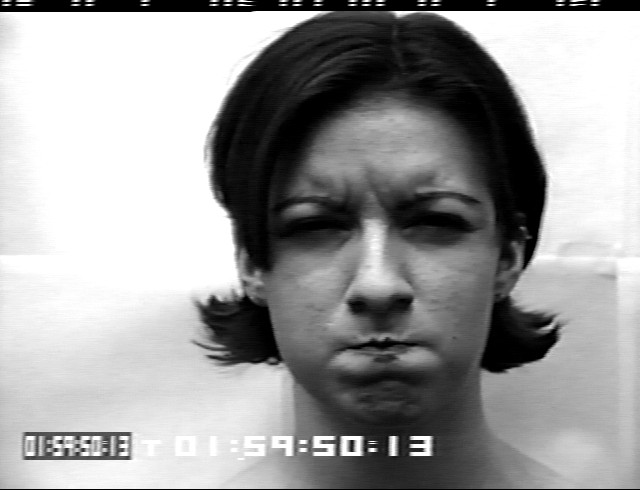
\includegraphics[width=.48\textwidth]{img/lec5f/S010_004_00000019.png}%
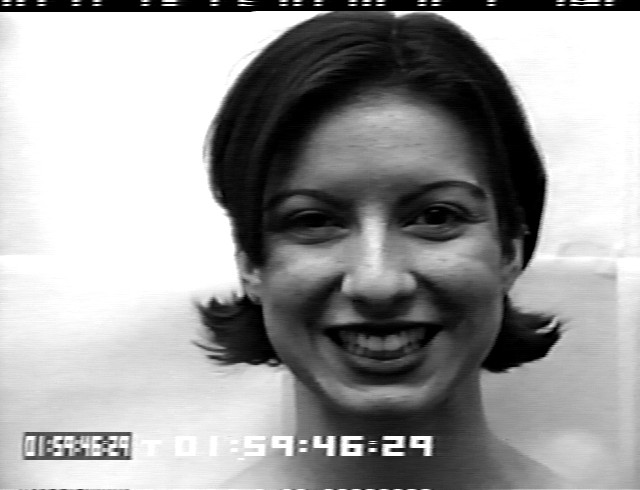
\includegraphics[width=.48\textwidth]{img/lec5f/S010_006_00000015.png}

\bigskip Each picture is labelled with one of the following emotion: anger, contempt, disgust, fear, happiness, sadness, and surprise.
    
\end{frame}
%\begin{frame}{Active Appearance Models}

Each pictures is processed with Active Appearance Models.

\bigskip Consider a cloud of 68 points representing some abstract face, in which each point (\emph{landmark point}) is some particular point of the face.

\bigskip\centering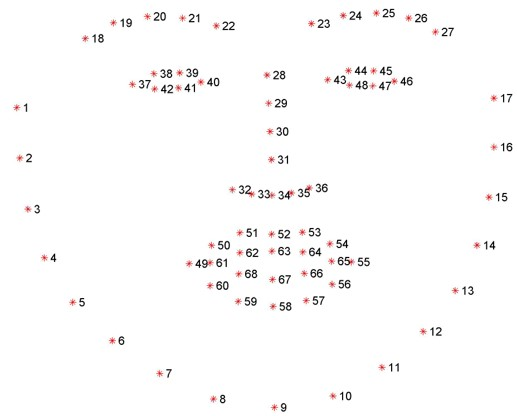
\includegraphics[width=.5\textwidth]{img/lec5f/template.jpg}
\end{frame}

\begin{frame}{Active Appearance Models (2)}
The cloud of points is deformed in order to stick with the face in the picture.

\bigskip\centering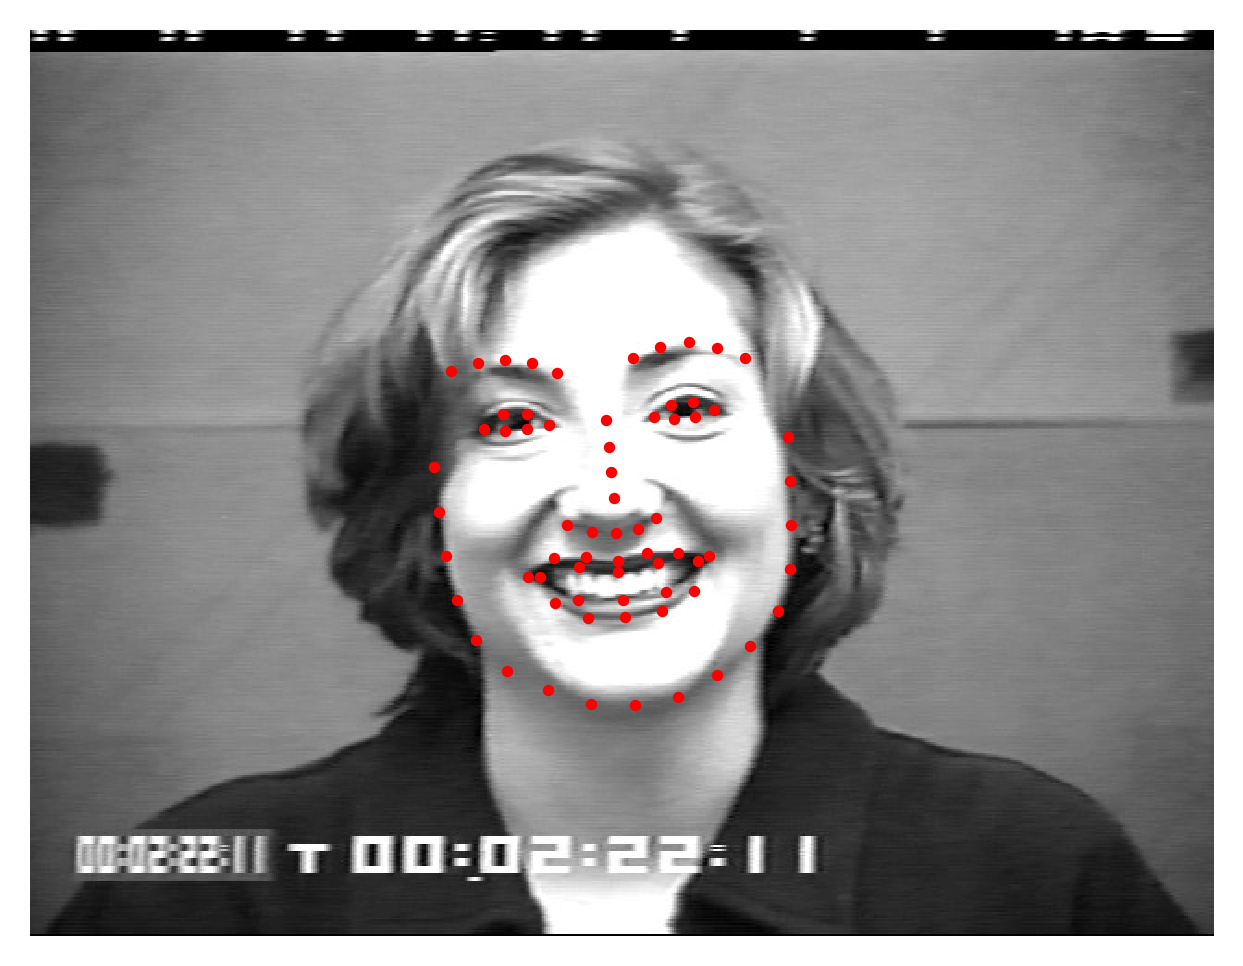
\includegraphics[width=.6\textwidth]{img/lec5f/S046_005_00000023.png}
\end{frame}
%\begin{frame}{Faces \(\to\) graphs}

We keep only point related to the mouth. 

\bigskip In order to obtain a \textit{weighted graph} from the previous data cloud we opted for two different strategies:

\only<1>{

\begin{itemize}
	\item \textbf{Complete graph} whose vertices are the landmark points of the mouth and  edge-weights $ w_{ij} $ are equal to  the Euclidean distance between vertices $ i $ and $ j $.
\end{itemize}	

\bigskip\centering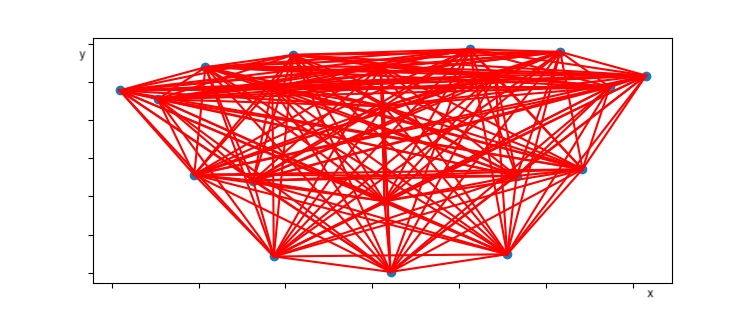
\includegraphics[width=0.5\textwidth]{img/lec5f/boccacomplete.png}}

\only<2>{

\begin{itemize}
	\item \textbf{Meshed graph} obtained using  the Delaunay triangulation algorithm of the  mouth  landmark points (complexity $ O(n \log n) $), also in this case the   edge-weights $ w_{ij} $ are equal to  the Euclidean distance between vertices $ i $ and $ j $.
\end{itemize}	

\bigskip\centering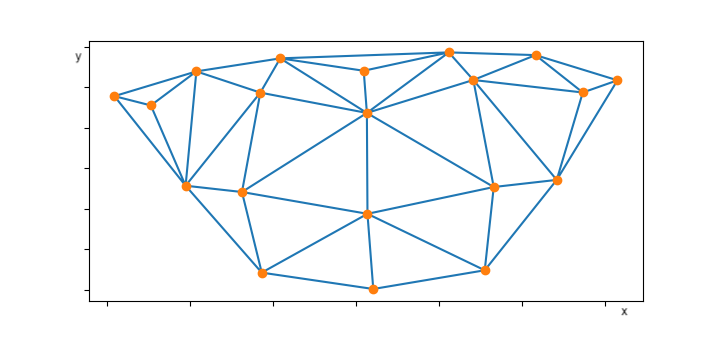
\includegraphics[width=0.5\textwidth]{img/lec5f/boccamesh.png}}

\end{frame}

\begin{frame}{Graph representation}

The graph is represented through its adjacency matrix.

\bigskip We keep only the upper triangular without diagonal, since the graph is undirected (symmetric matrix) and without self loop (the distance between any point with itself is zero). 

\bigskip Vectorize the matrix.

\end{frame}
\begin{frame}{Classical classifier}

The classifier receives in input the vector $x_\text{test}$ and two vectors $x_0, x_1$ which are one representative of the happy and sad faces.

\bigskip The Euclidian distances $\mathrm{distance}(x_\text{test}, x_0)$ and $\mathrm{distance}(x_\text{test}, x_1)$ are calculated. The test instance is classifies as the closest representative, whose distance is lower. 

\end{frame}

\begin{frame}[fragile]{The code}

\begin{minted}{python}
def classical_distance(G_0, G_1, G_test, tol=0.00001):
    
    # distance between the test instance and the happy instance
    distance_0 = np.linalg.norm(G_0 - G_test)
    # distance between the test instance and the sad instance
    distance_1 = np.linalg.norm(G_1 - G_test)
    # the difference is = 0 if the distance is equal, > 0 if sad is closest, < 0 if happy is closest
    difference = distance_0 - distance_1
    # remove some numerical error that can classify numbers like +-0.00001 as Y1 or Y0 instead of EQUALS
    the_difference = 0 if np.abs(difference) <= tol else difference
    
    # sign(difference) = 0 -> EQUAL; sign(difference) = 1 -> Y1; sign(difference) = -1 -> Y0
    label = int(np.sign(the_difference))
    return difference, ["EQUAL", "Y1", "Y0"][label]
\end{minted}
\end{frame}



\begin{frame}{Quantum classifier}
    \begin{center}
        \scalebox{0.8}{\begin{quantikz}[]
    \lstick{\(\ket{0}_a\)}\qw
        & \gate{H}
        & \ctrl{2}
        & \gate{X}
        & \ctrl{2}
        & \qw
        & \ctrl{2}
        & \gate{H}
        & \meter{\text{discard }1}
        & \cwbend{3}
        & \cw \rstick{a} \\
    \lstick{\(\ket{0}_i\)}\qw
        & \gate{H}
        & \qw
        & \qw
        & \ctrl{1}
        & \gate{X}
        & \ctrl{1} 
        & \ctrl{2}
        & \qw
        & \qw & \qw \\
    \lstick{\(\ket{0\cdots 00}_g\)}\qw
        & \qw
        & \gate{\mathbf{G_\text{\textbf test}}}
        & \qw
        & \gate{\mathbf{G^{\{1\}}}}
        & \qw
        & \gate{\mathbf{G^{\{2\}}}}
        & \qw
        & \qw
        & \qw & \qw \\
    \lstick{\(\ket{0}_c\)}\qw
        & \qw
        & \qw
        & \qw
        & \qw
        & \qw
        & \qw
        & \targ{}
        & \qw
        & \meter{}
        & \cw\rstick{c}
\end{quantikz}}
    \end{center}
\end{frame}

\begin{frame}{Quantum classifier}
The circuit evolves as it follows:
\only<1>{\begin{itemize}
\item the circuit starts in state:
$$|0\rangle_a |0\rangle_i |0\rangle_d |0\rangle_c;$$
\item after the first two Hadamard gates the state is:
$$\frac{1}{2} (|0\rangle+|1\rangle)_a (|0\rangle+|1\rangle)_i |0\rangle_d |0\rangle_c;$$
\end{itemize}
}%
%
\only<2>{\begin{itemize}
\item after the controlled initialization of the test instance the state is: 
$$\frac{1}{2} |0\rangle_a (|0\rangle+|1\rangle)_i |0\rangle_d |0\rangle_c
+ \frac{1}{2} |1\rangle_a (|0\rangle+|1\rangle)_i |G_\text{test}\rangle_d |0\rangle_c;$$
\item after the X operation on the ancilla qubit the state is:
$$\frac{1}{2} |0\rangle_a (|0\rangle+|1\rangle)_i |G_\text{test}\rangle_d |0\rangle_c
+ \frac{1}{2} |1\rangle_a (|0\rangle+|1\rangle)_i |0\rangle_d |0\rangle_c;$$
\end{itemize}
}%
%
\only<3>{\begin{itemize}
\item after the double-controlled initialization of the first representative the state is:
$$\frac{1}{2} |0\rangle_a (|0\rangle+|1\rangle)_i |G_\text{test}\rangle_d |0\rangle_c
+ \frac{1}{2} |1\rangle_a |0\rangle_i |0\rangle_d |0\rangle_c
+ \frac{1}{2} |1\rangle_a |1\rangle_i |G_0\rangle_d |0\rangle_c;$$
\item after the X operation on the index register the state is:
$$\frac{1}{2} |0\rangle_a (|0\rangle+|1\rangle)_i |G_\text{test}\rangle_d |0\rangle_c
+ \frac{1}{2} |1\rangle_a |0\rangle_i |G_0\rangle_d |0\rangle_c
+ \frac{1}{2} |1\rangle_a |1\rangle_i |0\rangle_d |0\rangle_c;$$
\item after the double-controlled initialization of the second representative the state is:
$$\frac{1}{2} |0\rangle_a (|0\rangle+|1\rangle)_i |G_\text{test}\rangle_d |0\rangle_c
+ \frac{1}{2} |1\rangle_a |0\rangle_i |G_0\rangle_d |0\rangle_c
+ \frac{1}{2} |1\rangle_a |1\rangle_i |G_1\rangle_d |0\rangle_c;$$
\end{itemize}
}%
%
\only<4>{\begin{itemize}
\item after the CNOT gate binding the index register with the class register, the state is:
{\footnotesize $$\frac{1}{2} |0\rangle_a |0\rangle_i |G_\text{test}\rangle_d |0\rangle_c
+ \frac{1}{2} |0\rangle_a |1\rangle_i |G_\text{test}\rangle_d |1\rangle_c
+ \frac{1}{2} |1\rangle_a |0\rangle_i |G_0\rangle_d |0\rangle_c
+ \frac{1}{2} |1\rangle_a |1\rangle_i |G_1\rangle_d |1\rangle_c;$$}%

for the sake of visualization, we set $|0\rangle_c$ as $|y_0\rangle_c$ and $|1\rangle_c$ as $|y_1\rangle_c$ to remind us that such register contains the two labels:
{\footnotesize $$\frac{1}{2} |0\rangle_a |0\rangle_i |G_\text{test}\rangle_d |y_0\rangle_c
+ \frac{1}{2} |0\rangle_a |1\rangle_i |G_\text{test}\rangle_d |y_1\rangle_c
+ \frac{1}{2} |1\rangle_a |0\rangle_i |G_0\rangle_d |y_0\rangle_c
+ \frac{1}{2} |1\rangle_a |1\rangle_i |G_1\rangle_d |y_1\rangle_c;$$}
which is re-arranged into the following equation:
$$ \frac{1}{2} \sum_{k \in \{0, 1\}} \Big( |0\rangle_a |G_\text{test}\rangle_d + |1\rangle_a |G_k\rangle_d  \Big) |k\rangle_i |y_k\rangle_c;$$
\end{itemize}
}%
%
\only<5>{\begin{itemize}
\item after the final Hadamard gate the state is: $$\frac{1}{2\sqrt{2}} \sum_{k \in \{0, 1\}} \Big( |0\rangle_a (|G_\text{test}\rangle + |G_k\rangle)_d + |1\rangle_a (|G_\text{test}\rangle - |G_k\rangle)_d \Big) |k\rangle_i |y_k\rangle_c.$$
\end{itemize}}
\end{frame}

\begin{frame}{Measurement interpretation}

By estimating the probability of reading class $y_0=0$ or $y_1=1$ we can estimate the distance between $G_\text{test}, G_0$ with respect to the distance between $G_\text{test}, G_1$. So, 

$$y_\text{test} = \begin{cases}
    y_0,           & > .5 \\
    y_1,           & < .5 \\
    \text{equals}, & = .5
\end{cases}$$

To mitigate the errors due to the probabilistic nature of the computation, we can introduce a small tollerance $\epsilon$ around the boundary between the two labels:

$$y_\text{test} = \begin{cases}
    y_0, & > .5+\epsilon \\
    y_1, & < .5-\epsilon \\
    \text{equals}, & \text{otherwise}
\end{cases}$$
\end{frame}
\begin{frame}[fragile]{Your turn!}
\begin{minted}{python}
def quantum_distance(G_0, G_1, G_test, tol=0.00001):
    # ...
    return difference, label
\end{minted}
\end{frame}

\begin{frame}[fragile]{Test the correctness}
\begin{minted}{python}
def test_accuracy_of_classification(states):
    correct, wrong = 0, 0
    for i, first_data in enumerate(states):
        for j, second_data in enumerate(states):
            for k, third_data in enumerate(states):
                dc, cl = classical_distance(first_data,
                    second_data, third_data)
                dq, ql = quantum_distance(first_data,
                    second_data, third_data, tol=0.015)
                if cl == ql:
                    correct += 1
                    print(".", end="")
                else:
                    wrong += 1
                    print("X", end="")
    return (correct, wrong)
\end{minted}
\end{frame}

\begin{frame}[fragile]{Test the correctness}
\begin{minted}{python}
# create some quantum states
zero  = np.array([1, 0])
one   = np.array([0, 1])
plus  = (1/np.sqrt(2)) * np.array([1, 1])
minus = (1/np.sqrt(2)) * np.array([1, -1])
ipos  = (1/np.sqrt(2)) * np.array([1, complex(0,1)])
ineg  = (1/np.sqrt(2)) * np.array([1, complex(0,-1)])

# run the test
states = [zero, one, plus, minus, ipos, ineg]
correct, wrong = test_accuracy_of_classification(states)

# print results
print(f"\nClassified {correct} correctly and {wrong} wrongly")
\end{minted}
\end{frame}

\begin{frame}{Your turn!}
Download the starter code. The file \code{dataset.json} contains 26 elements, representing the path of an image, a path of its file containing the landmark points and its label. 

\bigskip Estimate the accuracy of both classical and quantum classifier. 
\end{frame}

%\section{Lecture 6: Quantum Approximate Optimization Algorithm}
\SectionPage{}

\section{Hamiltonian for Max-Cut}
\SectionPage{}

\begin{frame}{Max-Cut}
\begin{center}
    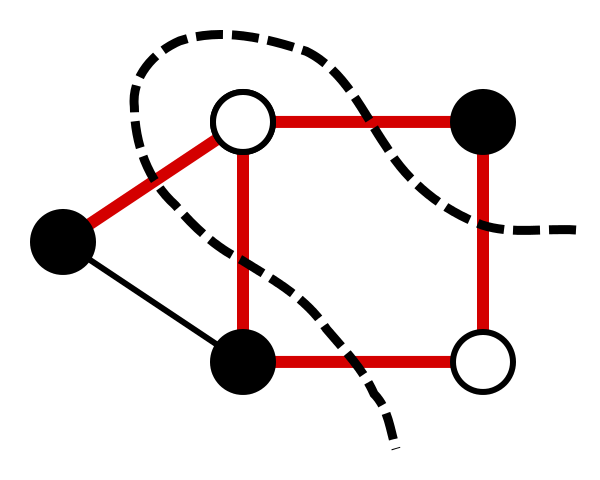
\includegraphics[width=0.5\textwidth]{img/lec6/Max-cut.svg.png}
\end{center}
\begin{itemize}
    \item one variable \( s_i \) per vertex
    \item \(s_i\) can take values \( -1, +1 \) 
\end{itemize}
\[ \text{MaxCut}(s_1, ..., s_n) = \max\frac{1}{2} \sum\limits_{(s_i, s_j) \in E} (1 - s_i s_j) \]
\end{frame}

\begin{frame}{Hamiltonian for MaxCut}
\begin{align*}
    \text{MaxCut}(s_1, ..., s_n) 
    & = \max\frac{1}{2} \sum\limits_{(s_i, s_j) \in E} (1 - s_i s_j) \\
    & = \max\frac{1}{2} \sum\limits_{(s_i, s_j) \in E} (- s_i s_j) + \text{const} \\
    & \equiv \max\sum\limits_{(s_i, s_j) \in E} (- s_i s_j) \\
    & \equiv \min\sum\limits_{(s_i, s_j) \in E} s_i s_j
\end{align*}
\end{frame}

\begin{frame}{Hamiltonian for MaxCut}
Map \(s_i\) to an operator that has 
\begin{itemize}
    \item eigenvalue \(+1\) associated to \(\ket{0}\);
    \item eigenvalue \(-1\) associated to \(\ket{1}\);
\end{itemize}

This operator is \(Z\). \bigskip

\[ H = \sum\limits_{(s_i, s_j) \in E} Z_i Z_j \]

\alert{Your turn}: create the Hamiltonian analytically for graph having vertexes \(V = \{v_1, v_2, v_3\}\) and edges \(E=\{(v_1, v_2); (v_2, v_3)\}\). 

\begin{center}
    \begin{tikzpicture}
    \node (v1) at (0,0) {\(v_1\)};
    \node (v2) at (1,1) {\(v_2\)};
    \node (v3) at (2,0) {\(v_3\)};
    \draw (v1) -- (v2) -- (v3);
    \end{tikzpicture}
\end{center}

\end{frame}

\begin{frame}[fragile]{Hamiltonian for MaxCut}
\begin{minted}{python}
import numpy as np
Z = np.array([[1, 0], [0, -1]])
I = np.array([[1, 0], [0, 1]])
H = np.kron(np.kron(Z, Z), I) # Z_1 Z_2
H += np.kron(I, np.kron(Z, Z)) # Z_2 Z_3
# array([[ 2,  0,  0,  0,  0,  0,  0,  0],
#        [ 0,  0,  0,  0,  0,  0,  0,  0],
#        [ 0,  0, -2,  0,  0,  0,  0,  0],
#        [ 0,  0,  0,  0,  0,  0,  0,  0],
#        [ 0,  0,  0,  0,  0,  0,  0,  0],
#        [ 0,  0,  0,  0,  0, -2,  0,  0],
#        [ 0,  0,  0,  0,  0,  0,  0,  0],
#        [ 0,  0,  0,  0,  0,  0,  0,  2]])
\end{minted}

Solution associated to \(\ket{010}\), \(\ket{101}\) has minimum valued eigenvalues.
\end{frame}

\section{The goal}
\SectionPage{}

\begin{frame}{The goal}
\emph{Goal}: minimize a cost function \(C\).
\begin{itemize}
    \item<2-> NP-Hard
    \item<3-> Exhaustive search vs heuristics
\end{itemize}
\end{frame}

\begin{frame}{Variational quantum circuits}
Some ideas:
\begin{itemize}
    \item<1-> Quantum circuit as a parametric model;
    \item<2-> Parameters optimized classically. 
\end{itemize}
\end{frame}

\begin{frame}{QAOA}
Steps:
\begin{enumerate}
    \item<1-> define your problem in terms of an Hermitian matrix \(H\), the solution of your problem must coincide with the ground state of \(H\) (eigenvector associated with the minimum valued eigenvalue).
    \begin{itemize}
        \item<2-> we consider only \(H\) diagonal;
        \item<3-> ground state: row (equiv. column) of the computational basis associated to the minimum valued eigenvalue;
        \item<4-> all solutions are from computational basis = retrieve them with certainty.
    \end{itemize}
    \item<5-> build the unitary circuit \(U = e^{iH}\) and make it parametric with a single parameter \(\gamma\): \(U_\gamma = e^{i\gamma H}\);
    \item<6-> build the unitary \(U_\beta\) given by rotating \(\text{Rx}(\beta)\) on any qubit;
    \item<7-> the whole circuit is: \(H^{\otimes n}\) then repeat \(U_{\gamma_i} U_{\beta_i}\) p-times.
\end{enumerate}
\end{frame}


\begin{frame}{QAOA}
\begin{center}
    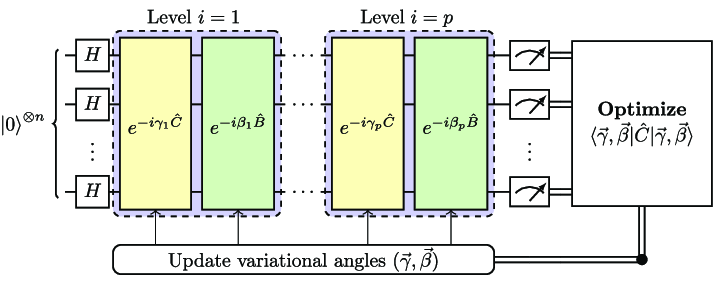
\includegraphics[width=\textwidth]{img/lec6/qaoa.png}
\end{center}
\end{frame}


\begin{frame}{QAOA}
\alert{Note}: no guarantees of performance improvement. 
\end{frame}


\begin{frame}{QAOA}
\alert{Note}: this tutorial is partially inspired by "A tutorial on Quantum Approximate Optimization Algorithm" 

\bigskip\begin{center}\url{youtube.com/watch?v=AOKM9BkweVU}\end{center}

\bigskip Covers much more!
\end{frame}

\section{The QAOA circuit}
\SectionPage{}

\begin{frame}{The Cost operator}
Implement the circuit \(U_\gamma = e^{i\gamma H}\). The interactions \(\gamma ZZ\) are performed by the circuit:
\begin{center}
    \begin{quantikz}
    \qw & \ctrl{1} & \qw                & \ctrl{1} & \qw \\
    \qw & \targ{}  & \gate{Rz(2\gamma)} & \targ{}  & \qw \\
    \end{quantikz}
\end{center}

\alert{Your turn}: check the math by comparing the result given by multiplying analytically \(\gamma Z \otimes Z\) as \code{gamma*np.kron(Z,Z)} and implementing this circuit and retrieving the unitary with \code{unitary\_simulator}.
\end{frame}

\begin{frame}{The Mixing operator}
Implement the circuit \(U_\beta\):
\begin{center}
    \begin{quantikz}
    \qw & \gate{Rx(2*\beta)} & \qw \\
    \qw & \gate{Rx(2*\beta)} & \qw 
    \end{quantikz}
\end{center}
\end{frame}

\begin{frame}{The QAOA circuit for \(p=1\)}
Implement the circuit \(U_\beta\):
\begin{center}
    \begin{quantikz}
    \lstick{\(\ket{0}\)} \qw & \gate{H} & \gate[wires=2]{\gamma_1 ZZ} & \qw & \gate{Rx(2\beta_1)} & \meter{} \\
    \lstick{\(\ket{0}\)} \qw & \gate{H} & \qw & \gate[wires=2]{\gamma_1 ZZ} & \gate{Rx(2\beta_1)} & \meter{} \\
    \lstick{\(\ket{0}\)} \qw & \gate{H} & \qw & \qw & \gate{Rx(2\beta_1)} & \meter{} 
    \end{quantikz}
\end{center}

The state at the end of this circuit is sometimes denoted with \(\ket{\vec{\gamma}, \vec{\beta}}\).
\end{frame}

\begin{frame}[fragile]{Parametrized circuits in QISKIT}
\begin{minted}{python}
from qiskit.circuit import Parameter
alpha = Parameter('a')
beta = Parameter('b')

qaoa_circuit = QuantumCircuit(1, 1)
qaoa_circuit.rx(alpha, 0)
qaoa_circuit.rx(beta, 0)
qaoa_circuit.measure(0, 0)

qc = qaoa_circuit.bind_parameters({
    alpha: 0.123, beta: 0.456})
\end{minted}
\end{frame}

\section{Measure interpretation}
\SectionPage{}

\begin{frame}[fragile]{Classical cost function}
Define the classical cost function for MaxCut:

\begin{minted}{python}
def cost_function(solution):
    cuts = 0
    # hardcode edges variable into this function 
    # or reference from the outside
    for (i, j) in edges:
        is_edge_cut = solution[i] != solution[j]
        if is_edge_cut:
            cuts += 1;
    return cuts
\end{minted}
\end{frame}

\begin{frame}[fragile]{Estimate the energy from the samples}
Estimate the energy for parameters \(\gamma, \beta\). This is sometimes denoted with \(\expval{C}{\vec{\gamma}, \vec{\beta}}\) where \(C\) is the classical cost function. \bigskip

\begin{minted}{python}
def estimate_energy(params):
    gamma_1 = params[0], beta_1 = params[1]
    # build circuit qc
    # ...
    SHOTS = 10000
    counts = execute(qc, qasm_sim, shots=SHOTS)
        .result().get_counts()
    # NOTE: invert the order of measurements
    mean_energy = 0
    for measure, freq in counts.items():
        mean_energy += cost_function(measure)*freq/SHOTS
    return mean_energy
\end{minted}
\end{frame}

\section{Optimization phase}
\SectionPage{}

\begin{frame}[fragile]{Optimization phase}
\begin{minted}{python}
from scipy.optimize import minimize
x0 = np.array([0.1, 0.2])
bnds = ((0,2*pi),)*2
res = minimize(estimate_energy, x0, method='COBYLA', bounds=bnds)

print("Best mean energy: ", estimate_energy(res.x))
print("Best gamma, beta: ", res.x)
\end{minted}
\end{frame}


\begin{frame}[fragile]{Optimization phase}
Execute one last time with the best parameters:\bigskip

\begin{minted}{python}
qc = qaoa_circuit.bind_parameters({
    gamma: res.x[0], beta: res.x[1]})
counts = execute(qc, Aer.get_backend("qasm_simulator"), 
    shots=SHOTS).result().get_counts()
best_solution = None
for solution, freq in counts.items():
    if best_solution == None:
        best_solution = solution
    if freq > counts[best_solution]:
        best_solution = solution
print("Best solution is: ", best_solution)
\end{minted}
\end{frame}





\section{Your turn}
\SectionPage{}

\begin{frame}{Your turn}
\begin{enumerate}
    \item Try QAOA with the MaxCut problem;
    \item Try QAOA with the 3-SAT problem;
    \begin{itemize}
        \item \alert{Hint}: since variables \(x_i\) in 3-SAT does not belong to \(\{\pm 1\}\) but they belong to \(\{0, 1\}\) we cannot map directly \(x_i \to Z_i\) but \(x_i \to \cdots\) (operator having eigenvalue 0 associated to \(\ket{0}\) and eigenvalue 1 associated to \(\ket{1}\)). 
    \end{itemize}
    \item Other problems: \url{https://arxiv.org/pdf/1302.5843.pdf}.
\end{enumerate}
\end{frame}

\end{document}